% Options for packages loaded elsewhere
\PassOptionsToPackage{unicode}{hyperref}
\PassOptionsToPackage{hyphens}{url}
%
\documentclass[
]{book}
\usepackage{lmodern}
\usepackage{amssymb,amsmath}
\usepackage{ifxetex,ifluatex}
\ifnum 0\ifxetex 1\fi\ifluatex 1\fi=0 % if pdftex
  \usepackage[T1]{fontenc}
  \usepackage[utf8]{inputenc}
  \usepackage{textcomp} % provide euro and other symbols
\else % if luatex or xetex
  \usepackage{unicode-math}
  \defaultfontfeatures{Scale=MatchLowercase}
  \defaultfontfeatures[\rmfamily]{Ligatures=TeX,Scale=1}
\fi
% Use upquote if available, for straight quotes in verbatim environments
\IfFileExists{upquote.sty}{\usepackage{upquote}}{}
\IfFileExists{microtype.sty}{% use microtype if available
  \usepackage[]{microtype}
  \UseMicrotypeSet[protrusion]{basicmath} % disable protrusion for tt fonts
}{}
\makeatletter
\@ifundefined{KOMAClassName}{% if non-KOMA class
  \IfFileExists{parskip.sty}{%
    \usepackage{parskip}
  }{% else
    \setlength{\parindent}{0pt}
    \setlength{\parskip}{6pt plus 2pt minus 1pt}}
}{% if KOMA class
  \KOMAoptions{parskip=half}}
\makeatother
\usepackage{xcolor}
\IfFileExists{xurl.sty}{\usepackage{xurl}}{} % add URL line breaks if available
\IfFileExists{bookmark.sty}{\usepackage{bookmark}}{\usepackage{hyperref}}
\hypersetup{
  pdftitle={Phylogenetic Biology},
  pdfauthor={Casey W. Dunn},
  hidelinks,
  pdfcreator={LaTeX via pandoc}}
\urlstyle{same} % disable monospaced font for URLs
\usepackage{longtable,booktabs}
% Correct order of tables after \paragraph or \subparagraph
\usepackage{etoolbox}
\makeatletter
\patchcmd\longtable{\par}{\if@noskipsec\mbox{}\fi\par}{}{}
\makeatother
% Allow footnotes in longtable head/foot
\IfFileExists{footnotehyper.sty}{\usepackage{footnotehyper}}{\usepackage{footnote}}
\makesavenoteenv{longtable}
\usepackage{graphicx,grffile}
\makeatletter
\def\maxwidth{\ifdim\Gin@nat@width>\linewidth\linewidth\else\Gin@nat@width\fi}
\def\maxheight{\ifdim\Gin@nat@height>\textheight\textheight\else\Gin@nat@height\fi}
\makeatother
% Scale images if necessary, so that they will not overflow the page
% margins by default, and it is still possible to overwrite the defaults
% using explicit options in \includegraphics[width, height, ...]{}
\setkeys{Gin}{width=\maxwidth,height=\maxheight,keepaspectratio}
% Set default figure placement to htbp
\makeatletter
\def\fps@figure{htbp}
\makeatother
\setlength{\emergencystretch}{3em} % prevent overfull lines
\providecommand{\tightlist}{%
  \setlength{\itemsep}{0pt}\setlength{\parskip}{0pt}}
\setcounter{secnumdepth}{5}
\usepackage{booktabs}
\usepackage[]{natbib}
\bibliographystyle{apalike}

\title{Phylogenetic Biology}
\author{Casey W. Dunn}
\date{2020-07-26}

\begin{document}
\maketitle

{
\setcounter{tocdepth}{1}
\tableofcontents
}
\hypertarget{preface}{%
\chapter*{Preface}\label{preface}}
\addcontentsline{toc}{chapter}{Preface}

I developed this book as a collection of the concepts, methods, and applications that I most wanted to share with students in my Phylogenetic Biology courses.

\hypertarget{intro}{%
\chapter{Introduction}\label{intro}}

Phylogenetic biology is the study of evolutionary relationships.

There are three components to a phylogenetic analysis: characters, evolutionary models, and phylogenetic trees. In any given study we could have data, not care, or want to infer any three of these.

When we don't care, we marginalize. When we have data we fix. When we want to infer we estimate.

This gives a broad range of hypothetical phylogenetic investigations. Only a subset of these are common in the literature, due to the questions that drive the field right now, the available data, and the methods that have been implemented in software tools.

When we want to infer phylogenetic trees, we usually fix the characters at the tips using our data, marginalize over historical character states, estimate models, and estimate the tree.

When we want to infer the history of character evolution, we often fix the tree, fix the characters at the tips using our data, estimate the model, and estimate the character history.

But we can also marginalize over models, for example.

\hypertarget{why-phylogenies-matter}{%
\section{Why phylogenies matter}\label{why-phylogenies-matter}}

History of life on earth

Phylogenetic systematics

Comparative methods

Processes of evolution

Current and future evolution (eg epidemiology)

\hypertarget{required-background}{%
\section{Required background}\label{required-background}}

Comfort at the command line, manipulation of text files. \emph{Practical Computing for Biologists}.

Basic literacy with the programming language R. \emph{R for Data Science}.

Basic statistics, in particular probability theory. Some math, in particular an understanding of matrices and manipulations of matrices.

\hypertarget{additional-resources}{%
\section{Additional resources}\label{additional-resources}}

\hypertarget{trees}{%
\chapter{Trees}\label{trees}}

\hypertarget{anatomy}{%
\section{Anatomy}\label{anatomy}}

Trees are a special find of graph. Bifurcating acyclic.

Nodes, edges (branches).

I'll stick with the mathematical convention of calling branches edges, since this makes for stronger conceptual ties to other fields that also consider graphs.

\hypertarget{types}{%
\section{Types}\label{types}}

Cladogram, phylogram, time tree

\hypertarget{interpretation}{%
\section{Interpretation}\label{interpretation}}

Tree thinking

\hypertarget{representation}{%
\section{Representation}\label{representation}}

paranthetical

ape

ggtree

\hypertarget{simulation}{%
\chapter{Simulation}\label{simulation}}

Build the machinery to simulate the evolution of traits on trees. Focus for now on DNA evolution.

\hypertarget{models}{%
\section{Models}\label{models}}

Generative models

The intent is a simplified representation of the process under consideration.

``All models are wrong, some are useful''

\hypertarget{a-simple-model}{%
\section{A simple model}\label{a-simple-model}}

Let's start with a simple model of DNA evolution. Imagine that when the DNA is being replicated, most of the time the appropriate nucleotide is incorporated. Some fraction of the time, at rate \(\mu\), an event occurs where the appropriate nucleotides is replaced with a random nucleotide instead. The probability of selecting any of the nucleotides during one of these random replacement events is uniform (picking a C is just as probably as picking a G, for example), and the new nucleotide doesn't depend in any way on what nucleotide was there before. It is as if you had a bag containing equal frequencies of C, G, T, and A nucleotides. As you built the new DNA strand, every so often you would replace the nucleotide you should be adding with one you instead selected by reaching into the bag with your eyes closed and picking one at random.

Not all replacement events will result in an apparent change. Sometimes the appropriate nucleotide is selected by chance, even though it was picked at random. If, for example, the appropriate nucleotide was an A, under this model \(1/4\) of the time a replacement event occurs an A is selected by chance and there is no apparent change. In such a case, there has not been a substitution (just a replacement in kind). If the A is replaced with any of the other three nucleotides we say there has been a substitution. Because three of the four possible outcomes of an event result in a substitution, the substitution rate is \(3\beta\), which, because \(\beta=\mu/4\), is equivalent to noting that the substitution is \((3/4) \mu\). Because some events result in no apparent change, substitutions are only a subset of events and the substitution rate is \emph{lower} than the replacement event rate.

It might seem a bit odd to consider replacement events that don't result in substitutions, but this follows naturally from a central feature we specified for the the model - the new nucleotide doesn't depend in any way on what nucleotide was there before. If we had a process where replacements always resulted in substitutions, then excluding the a replacement in kind would require knowing which nucleotide should be placed so that we \emph{don't} select it.

\hypertarget{expected-amount-of-change}{%
\subsection{Expected amount of change}\label{expected-amount-of-change}}

One of the primary values of a model is that it allows us to think explicitly about how much evolutionary change we expect to see under the specified process. For the simple process described here, there are two things to consider if we want to know the amount of evolutionary change. The first is the substitution rate \(\mu\) (which we also know if we know \(\beta\), since \(\mu=4\beta\)), and the time over which the evolutionary process acts.

In Figure \ref{fig:sim-jc-mu-sweep} the amount of evolutionary time is held constant, and the rate \(\mu\) is changed. When \(\mu=0\), the bottom bar, there are no replacements (black bars) and therefore no substitutions (the whole bar is the same color).

\begin{figure}
\centering
\includegraphics{phylogenetic_biology_files/figure-latex/sim-jc-mu-sweep-1.pdf}
\caption{\label{fig:sim-jc-mu-sweep}Each horizontal bar is a simulation of evolution of a single nucleotide position through time, \(t\), for a specified value of \(\mu\). Each sumulation starts out as an A. Black vertical bars correspond to replacement events, which don't all lead to substitutions (a new color).}
\end{figure}

As \(\mu=0\) increases (going up on the \(y\) axis), the number of replacement events over the same time interval increases (Figure \ref{fig:sim-jc-mu-n}). This reflects the simple linear relationship \(n=\mu t\), where \(n\) is the number of expected replacement events.

\begin{figure}
\centering
\includegraphics{phylogenetic_biology_files/figure-latex/sim-jc-mu-n-1.pdf}
\caption{\label{fig:sim-jc-mu-n}The number of replacement events increases linearly with the replacement rate \(\mu\). This plot is from the same simulation as that shown in Figure \ref{fig:sim-jc-mu-sweep}. The line is a linear model fit to the data.}
\end{figure}

Because of the linear relationship between the number of replacements and the product \(\mu t\), rate and time are conflated. In many scenarios you can't estimate them independently. If there are a small number of replacements, for example, you can't be sure if there is a low rate over a long time interval or a high rate over a short interval. Both would give the same result. Because they are so often confounded in phylogenetic questions, often the rate is essentially fixed at one and the unit of time for edge lengths is given as the number of expected evolutionary change rather than absolute time (years, months, etc). You will often see this length as the scale bar of published phylogenies (Figure \ref{fig:sim-tree-cnid}). The exception is when you have external information, such as dated fossils, that allow you to independently estimate edge lengths and rates.

\begin{figure}
\centering
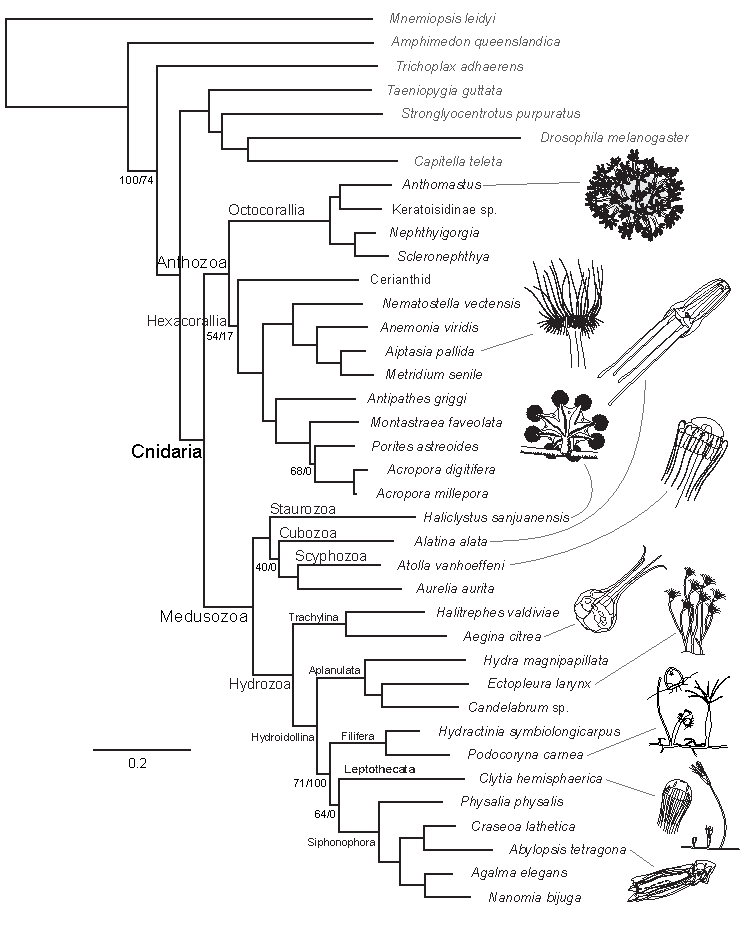
\includegraphics{figures/Fig_cnidaria.png}
\caption{\label{fig:sim-tree-cnid}A published phylogeny \citep{zapata2015} with a scale bar indicating branch length in terms of the expected amount of evolutionary change, rather than absolute time.}
\end{figure}

\hypertarget{expected-end-state}{%
\subsection{Expected end state}\label{expected-end-state}}

The machinery above shows how a model can clarify the way we think about the expected amount of change. Many times, though, we want to know what the probability of a given end state is given a starting state, a model, and the amount of time elapsed. One way to anchor such a question is to think about the extremes - what do we expect after a very small amount of change (either a short time or a slow rate of change, or both), and what do we expect after a large amount of change?

The situation is most clear after a small amount of change - we expect the end result to be the same as the starting condition. If we start with an A, for example, we expect to end with an A. In this situation, if we know the starting state that information tells us a lot about the end state. Not much else matters.

What should we expect, though, if there has been a large amount of change? Can we know anything at all? It turns out that we can. If there have been many replacements, one after the other, than the initial starting state really doesn't matter at all because whatever was there will probably have been replaced multiple times. If the starting state doesn't contain information about the end state, what does? It is the bag that you are picking the nucleotides at random from. Given enough evolutionary time, our simple model will lead the expected frequency of each nucleotide in the evolving sequence to be the same as the frequency in the bag that we randomly draw them from. Since we specified that you have the same chance of grabbing any nucleotide from the bag, eventually the probability of having each of the our nucleotides is the same, 25\%. If you started with a sequence that had an A and let it evolve 100 times, after enough evolutionary time had passed to reach equilibrium you would expect to get 25 C's, 25 G's, 25 T's, and 25 A's.

\begin{figure}
\centering
\includegraphics{phylogenetic_biology_files/figure-latex/sim-saturation-1.pdf}
\caption{\label{fig:sim-saturation}Stacked bar plots indicating the frequency of each nucleotide after evolution for a specified amount of time. The rate of evolution is \$\mu= 0.05 \$. There are 1000 replicate simulations for each value of time. At time=0 (no evolution), the end result is always the same as the initial value, which is fixed at A in these simulations. As the length of time increases, the four nucleotides converge on equal frequencies of 25\% each.}
\end{figure}

\hypertarget{generalizing-the-simple-model}{%
\section{Generalizing the simple model}\label{generalizing-the-simple-model}}

rates, equilibrium frequencies

\begin{verbatim}
##      [,1]
## [1,]    0
## [2,]    0
## [3,]    0
## [4,]    0
\end{verbatim}

exponentiation

\hypertarget{more-complex-models}{%
\section{More complex models}\label{more-complex-models}}

\hypertarget{model-structure}{%
\section{Model structure}\label{model-structure}}

\hypertarget{aditional-resources}{%
\section{Aditional resources}\label{aditional-resources}}

\begin{itemize}
\tightlist
\item
  My own thinking about this material was heavilly influenced by Paul Lewis's wonderful lectures at the annual Workshop on Molecular Evolution at Woods Hole. Some of his lectures are now available online as part of the excellent \href{https://www.youtube.com/channel/UCbAzhfySv7nLCrNYqZvBSMg}{Phylo Seminar}, starting with \url{https://www.youtube.com/watch?v=1r4z0YJq580\&t=2111s}
\end{itemize}

\hypertarget{inference}{%
\chapter{Inference}\label{inference}}

A specific task - given a set of character data corresponding to the tips of a tree, what is the topology of the tree? Model is also estimated, but may or may not be of interest.

Calculating the likelihood of a tree

What a likelihood is

maximum likelihood

hueristics

Bayesian

``Model free'' methods

\hypertarget{evaluation}{%
\chapter{Evaluation}\label{evaluation}}

\hypertarget{model-evaluation}{%
\section{Model evaluation}\label{model-evaluation}}

Why not add as many parameters as you can imagine?

Likelihood ratio test

AIC

BIC

\hypertarget{topology-evaluation}{%
\section{Topology evaluation}\label{topology-evaluation}}

\hypertarget{sensitiviy}{%
\section{Sensitiviy}\label{sensitiviy}}

changing methods and parameters

adding noise

\hypertarget{confidence}{%
\section{Confidence}\label{confidence}}

Propogation, point estimates

\hypertarget{epistemology}{%
\section{Epistemology}\label{epistemology}}

gene trees, species trees

\hypertarget{future}{%
\chapter{Future}\label{future}}

Integrated models of genome evolution

\hypertarget{shape}{%
\chapter{Shape}\label{shape}}

Dating

Diversification

Extinction, birth, death

Null models

\hypertarget{character-evolution}{%
\chapter{Character evolution}\label{character-evolution}}

Comparative biology

Reconstructing a single trait on trees

Trait correlation

Models of character change, including rate

\hypertarget{applications}{%
\chapter{Applications}\label{applications}}

\hypertarget{functional-genomic-data}{%
\section{Functional genomic data}\label{functional-genomic-data}}

\hypertarget{gene-trees}{%
\section{Gene trees}\label{gene-trees}}

  \bibliography{book.bib,packages.bib}

\end{document}
